\begin{itemize}
	\item first laser fabricated
	\item Created in 1960 by Maiman
	\item It is a 3 level system
	\item Produced light in pulsating maner (continuous mode not possible due to heating of active medium)
	\item Active medium: $\mathrm{Al}_{2} \mathrm{O}_{3} \cdot \mathrm{Cr}^{3+}$ (0.05-0.5 \% of Al atoms are replaced with Cr atoms)
	\item Pumping source: Xenon lamp. (the lamp has a helical structure that wounds the ruby rod).
	\item Eavelength of light emitted: 6943 $\amstr$
\end{itemize}

\begin{center}
	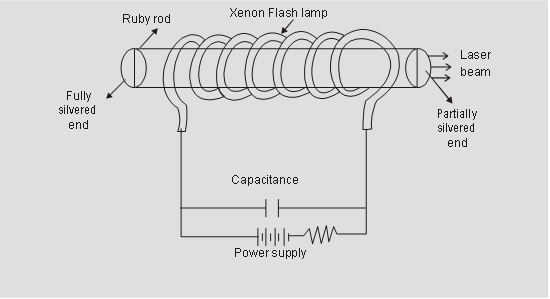
\includegraphics[max width=\textwidth]{ruby-laser}
\end{center}

$\star$ Population inversion is achieved between E$_m$ \& E,


\psset{algebraic,dimen=middle,linewidth=1.2pt,arrowsize=3pt 2,arrowinset=0.25}

\begin{pspicture*}(-.5,-1)(6.5,3.5)

	\psline{->}(0,0)(0,3)
	\psline{->}(0,0)(6.5,0)

	\rput[l](.15, 3){$E$}
	\rput[c](6.4, .4){$t$}

	\psplot[linewidth=1.5pt,linecolor=red,plotpoints=200]{0}{6}{1/(1+2.718281828^(-(x-0.5-PI/12)*15))*(SIN((x-0.5)*4-1.5)+1.2)*1/(1+2.718281828^((x-0.5-(4*PI)/3)*15-8))}

	\rput*[c](3.3,-.5){Intensity vs time graph}
\end{pspicture*}


\ussubsection{Working}
Cr$^{3+}$ ions absorb pumping light and go to excited states E$_2$ \& E$_3$. From these a rapid non-radiation transition to the metastable level E$_m$ takes place. Decay from E$_m$ is very slow that with sufficient excitation, populations inversion between E$_m$ \& E$_1$ can occur. Those photons are allowed to pass many times in the active medium with the help of mirrors. When threshold conditions are. satisfied, an intense pulse of light of wavelength 6934$\amstr$ is emitted. Continuous operation is not possible due to excessive heating of active medium.
